\documentclass[twoside,11pt]{article}
\usepackage[utf8]{jmlr2e}

\jmlrheading{Format}{2019}{5}{9/19}{9/19}{Assign1}{Peter Ottsen\u{a} and Bruce Clark\u{a} Justin McGowen\u{a} Forest Edwards}

\ShortHeadings{CSCI 447 Machine Learning Assignment 1}{{Ottsen, Clark, McGowen, Edwards}}

\begin{document}

\title{CSCI 447 Machine Learning Assignment 1}

\author{\name Peter Ottsen \email peter.k.ottsen@gmail.com\\
\name Bruce Clark \email brucewestonmt@gmail.com\\
\name Forest Edwards \email forestjedwards@gmail.com\\
\name Justin McGowen \email jmpanthers15@gmail.com}

\editor{None}

\maketitle

\begin{abstract}%

This paper contains the algorithm, experimental approach, results, and discussion of the first assignment.  Naive Bayes was the algorithm given for the assignment due to its relatively straightforward implementation. Five different data sets were used on the algorithm. Once the data sets were cleaned and processed, ten-fold cross-validation was used for each set and the accuracy and precision were recorded. Ten percent of the data in each data set was then scrambled and ten-fold cross-validation was again used with accuracy and precision being recorded.  The accuracy and precision of the scrambled vs non-scrambled data is discussed and theories for differences are offered.

\end{abstract}

\section{Problem Statement}

Problem statement including hypothesis

Searching for trends and patterns in data can prove to be quite a difficult and time-consuming challenge for data analysts, especially when they are dealing with very large amounts of data.  A more efficient method of analysis can be far more beneficial for finding data patterns.  The Naive Bayes algorithm can be very useful tool for this, as it can predict patterns in a dataset with high accuracy, by only using a small fraction of the data.  

In order to get a more accurate prediction for patterns in our data, we hypothesize that running the algorithm on the randomly scrambled data will be more accurate than running it on the ordered dataset.  We say this because a scrambled sample of data will be an unbiased, and more representative sample of the entire dataset.  This is important as it means that these randomized samples will be better at predicting patterns in the entire dataset.

\section{Description of Algorithm implemented}

The algorithm used in this assignment was Naive Bayes. Naive Bayes uses probabilities to develop a model to classify data based on its attributes. It is developed from Bayes Theorem:
\begin{center}
    $P(A|B) = \frac{P(A)*P(B|A)}{P(B)}$
\end{center}
$P(A|B)$ is the probability that A occurs if B occurs, $P(B|A)$ is the probability that B occurs if A occurs, and $P(A)$ \& $P(B)$ are the probability that A and B occur, respectively. (reference: An Elementary Introduction to Statistical Learning Theory). 

This theorem serves as the basis for the Naive Bayes Algorithm. This algorithm is  "naive" because the assumption is made that the attributes of each class are independent of each other. For example, this means that if a class consists of the attributes X, Y, Z the value of the X attribute has no effect on the value of the Y or Z attribute. This holds for each attribute. (reference:Machine Learning)

Below is a description of the steps for the training algorithm.  

First we calculate the fraction of the test data set made up by each of the classes, $c_i$, using the equation below. 
\begin{center}
    $Q(C=c_i) = \frac{#x\epsilon c_i}{N}$
\end{center}
This equation take the number of times class $i$ is seen and divides it by the total number of test data points, $N$.

Each respective class is then taken and the frequency of every attribute is calculated for that class using the below equation:
\begin{center}
    $F(A_j = a_k, C = c_i) = \frac{#\{x_{A_j} = a_k \wedge (x \epsilon c_i)\} + 1}{N_{c_i} + d} $
\end{center}
where F is the frequency of attribute $a_k$ for class $c_i$, $#\{x_{A_j} = a_k \wedge (x \epsilon c_i)\}$ is the number of times attribute $a_k$ show up in class $c_i$, $N_c_i$ is the number of times class $c_i$ shows up in the training data, and $d$ is the number of attributes. The $1$ is added at the top and $d$ is added on the bottom to smooth the data in case that attribute value does not exist for that class. 

From the results of the training algorithm above, the test data is then classified using the below equation:
\begin{center}
    $C(x) = Q(C=C_i) * \prod_{j=1}^d F(A_j = a_k, C = c_i)$
\end{center}
$C(x)$ is an array of values corresponding to the probabilities that the given test data belongs to each class. We then search for the class that has the highest relative probability value using the $argmax$ function:
\begin{center}
    $class(x) = argmax\ C(x)$
\end{center}
This class, $class(x)$, is then the predicted class for the test data.

\section{Experimental Approach}

The first thing we did when approaching this project was to examine the data and determined pre-processing was needed. The breast cancer data set was missing values so we randomly generated attribute values to fill them. The iris and glass data sets needed to be transformed into discrete values. We used the Gaussian distribution to split the attributes into four equally populated categories for these data sets.

Ten-fold cross-validation was used to test accuracy of the algorithm.  Each data set was split into ten sub-sets with equal proportions of each class. By splitting into equal portions, we are minimizing the potential for a class to be unrepresented in the training or test data. Nine of the ten sets were used to train the algorithm and the tenth was used to test the algorithm. This was done ten times over so that each sub-set served as the test data once. 

Data scrambling was used to test the resiliency of the algorithm. Once we tested the algorithm with ten-fold validation for each data set, ten percent of the data set was scrambled to have random values. These scrambled data sets were then tested on the algorithm using the same ten-fold validation method described above.   

The evaluation methods or loss function used were accuracy and precision. These were calculated creating a confusion matrix for each class and using the equations below:
\begin{center}
    $Accuracy = \frac{\#TruePositive + \#TrueNegative}{\# Of TestData}$\\
\end{center}

\begin{center}
    $Precision = \frac{\#TruePositive}{\#TruePositive + \#FalsePositive}$\\
\end{center}

\section{Results}

Presentation of the results of your experiments (in words, tables, and graphs)
We set out to try to figure out if introducing noise into a data set would improve the ability of our naive bayes algorithm. We tested our data sets with and without noise with a ten-fold cross-validation and with with a confusion matrix. The extensive results of these tests can be found in our results.txt folder in our folder. I will summarize the massive amounts of data generated by these data sets here.

In reguards to our ten-fold cross-validation, we averaged the accuracies and we found when testing the ten-fold cross-validation. We then averaged the accuracy between the classes here:


\begin{figure}[htp]
    \centering
    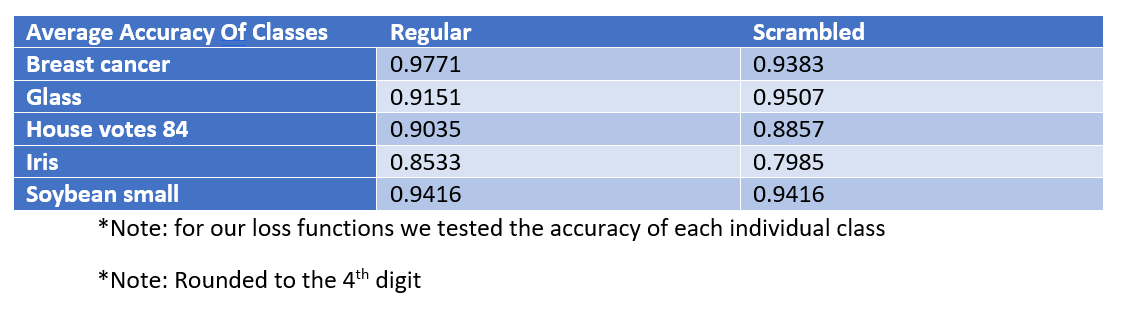
\includegraphics[width=10cm]{table1Accuracy.png}
\end{figure}


We can see that in general our scrambled data was less was less accurate than our regular data except in the glass dataset.

Taking a look at these results side by side shows differences in results we get upon scrambling our data. Here we can clearly see the differences between three important datasets.

\begin{center}
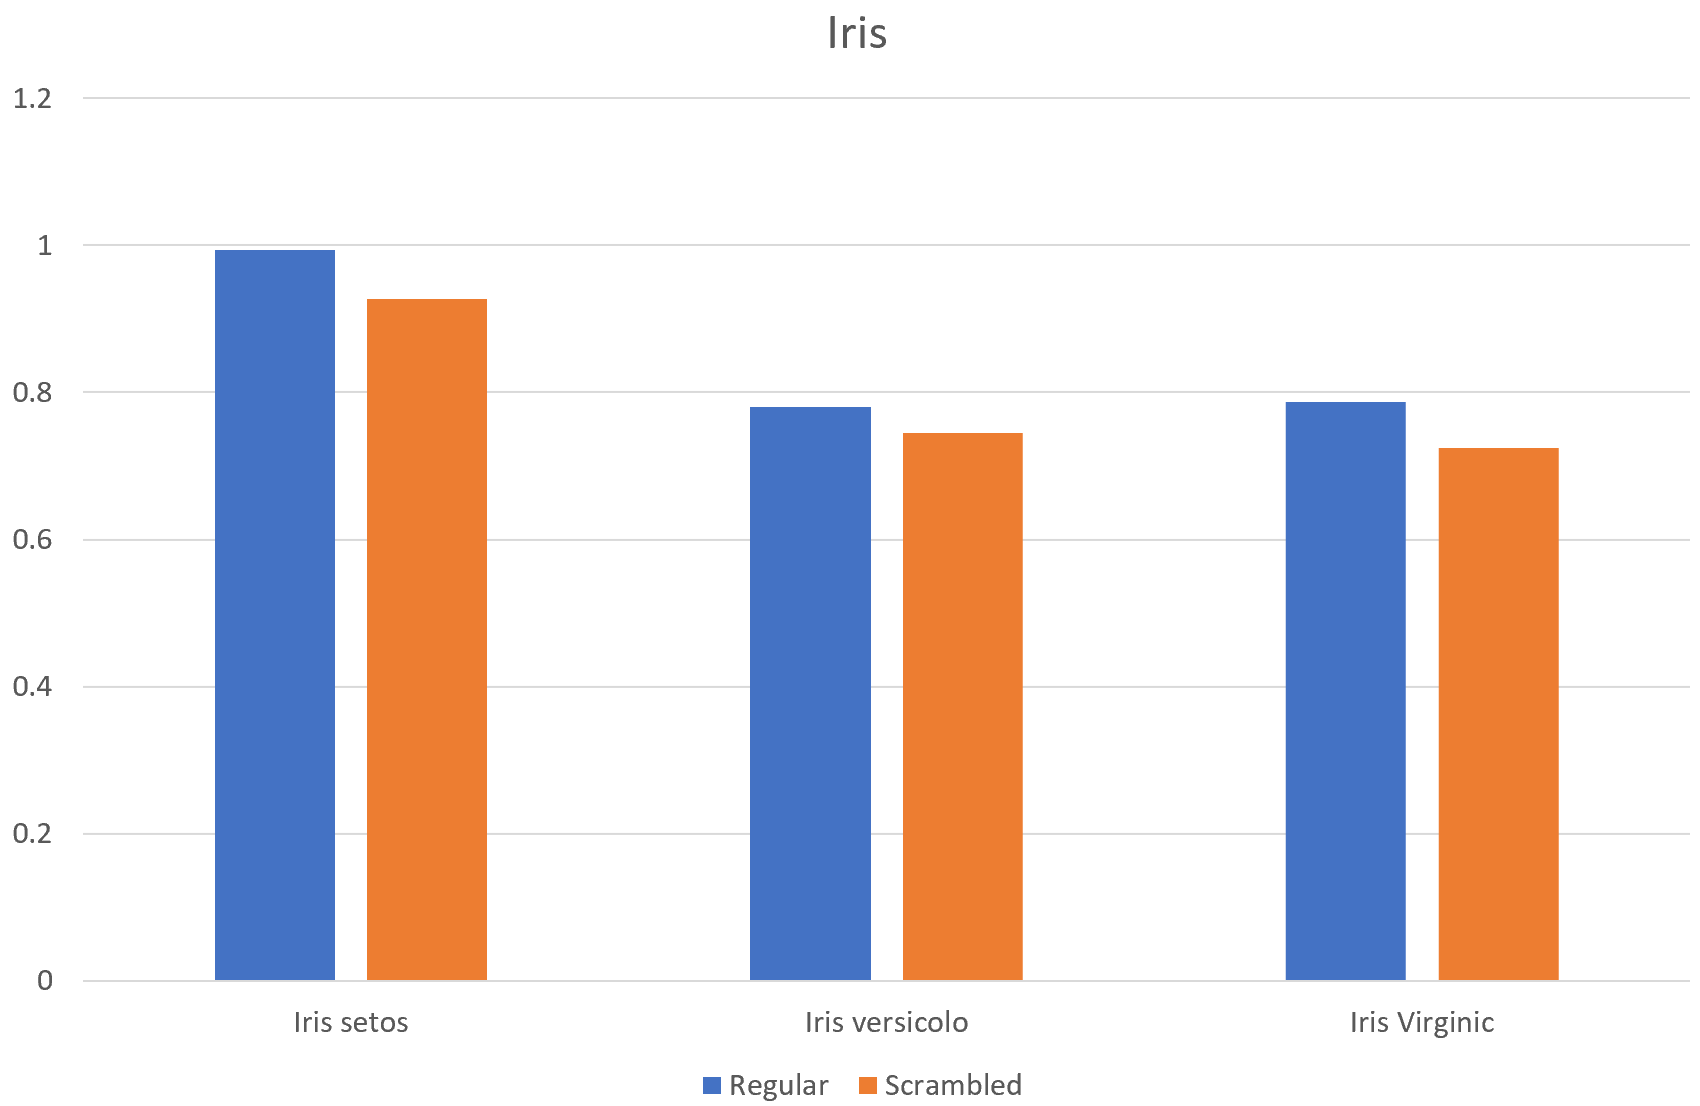
\includegraphics[width=10cm]{iris.png}
\end{center}
\begin{center}
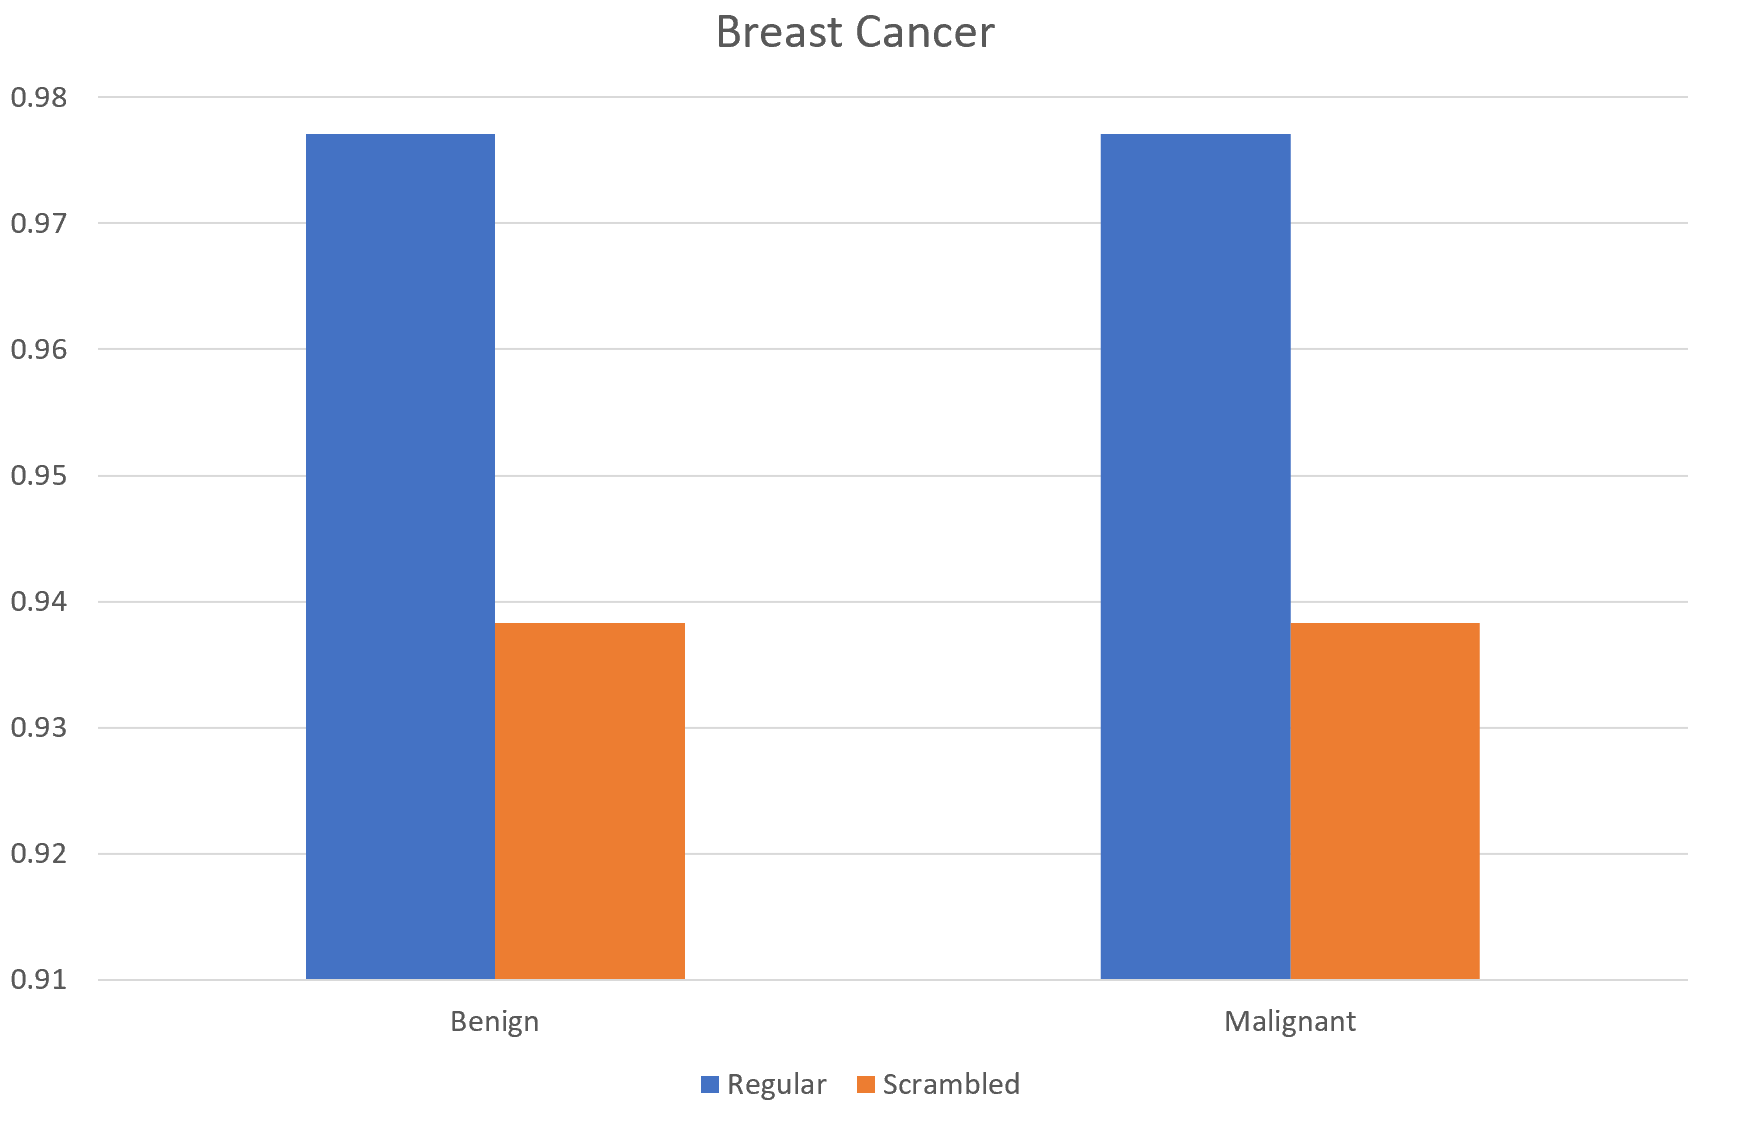
\includegraphics[width=10cm]{breastCan.png}


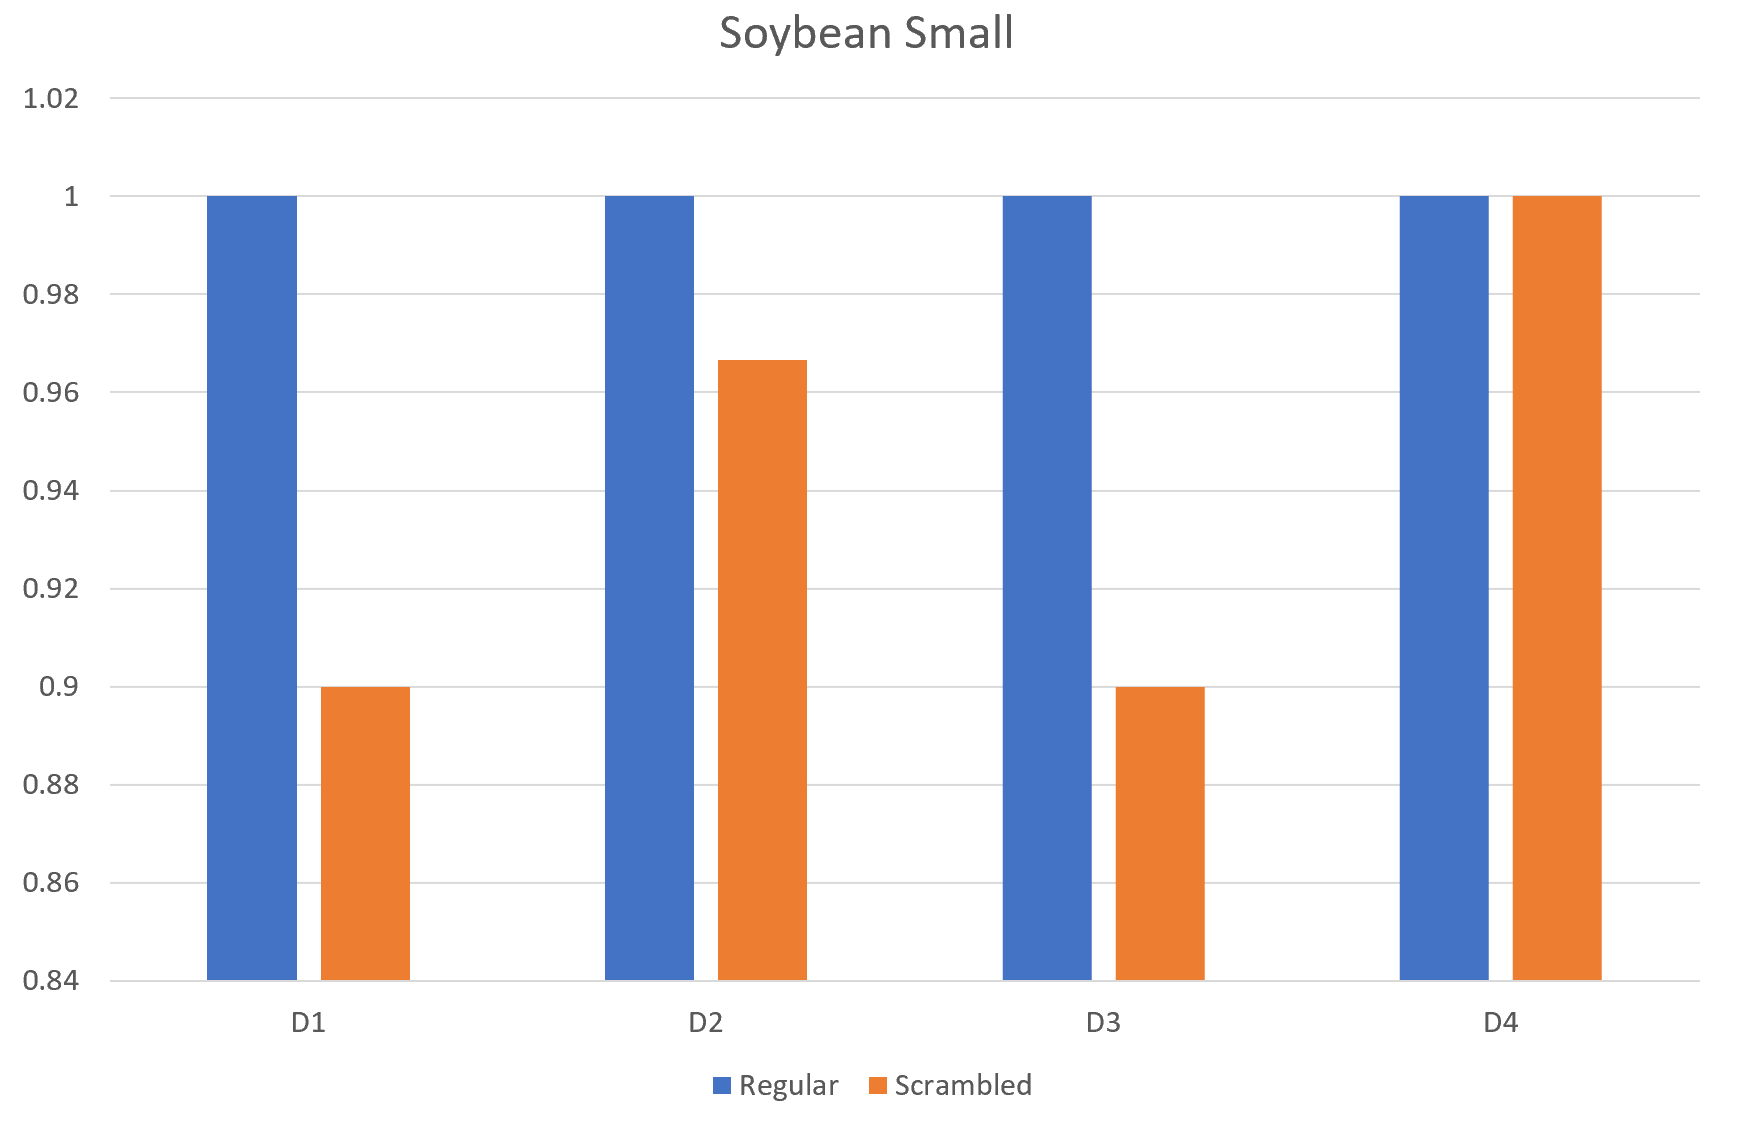
\includegraphics[width=10cm]{soybean.png}
\end{center}




\section{Discussion}

A discussion of the behavior of your algorithms, combined with any conclusions you can draw

Our algorithm usually had a slight decrease in effectively predicting the correct class when we introduced randomized data to our data set. When we introduced scrambled data, our data set would contain 10\% randomized data. What is interesting is that most of the time, the accuracy of predicting the classes of data sets with random data was not 10\% less than the accuracy of data that was not randomized.

Naive Bayes assumes classes and attributes are independent. We know that two of the three classes in Iris are not independent of each other. When predicting these classes, the class that is independent of the other two was predicted with over 90\% accuracy. What is surprising is that the two classes that are not linearly independent of each other were still able to be predicted with over 70\% accuracy.

In the soybeans data set, we noticed that some of the classes are strictly dependent on certain attributes. An example of this would be that attribute #26 is only value 2 when the class is D2. This was the set where our model was able to predict the class 100\% accurately. This leads us to draw the conclusion that this type of classification is more accurate when attributes have a stronger force on determining the class. 

This is also the data set where noise affected our data the most. We noticed up to a 10\% accuracy difference between our clean data and our data that introduced noise. This may lead to the conclusion that noise in attribute collection where these attributes strongly affect the class of this data is more crucial than when the attributes don't have a strong affect on the class. This could also lead to the conclusion that because multiple 

\section{Summary}

Summary

\section{References}

References

Data Sets:

Wolberg, William H. Dr. "Wisconsin Breast Cancer Database", January 8 1991.

German, B. "Glass Identification Database", September 1987.

Congressional Quarterly Almanac, 98th Congress, 2nd session 1984, Volume XL: Congressional Quarterly Inc. Washington, D.C., 1985. "1984 United States Congressional Voting Records Database", April 27 1987.

Fisher, R.A. "Iris Plants Database", July 1988.

Michalski,R.S. "Small Soybean Database", 1987.

“A Gentle Introduction to k-Fold Cross-Validation.” Machine Learning Mastery, 8 Aug. 2019, https://machinelearningmastery.com/k-fold-cross-validation/.

\end{document}
